\section{Resultater fra Affinity diagram}
\label{ParametreDatabehandlingAffinityDiagram}
%
Da formålet med projektet er, at udlede hvilke parametre danske rejsende tilskriver interaktionen med en social robot for efterfølgende at udvikle skalaer, som kan bruges til evaluere oplevelsen af interaktionen med robotten, bør der fremsættes nogle krav for hvordan parametrene udvælges for dernæst at formulere dem til skalaer. 

For at udlede parametrene fokuseres der på én grøn kategori af gangen, hvorfra parametrene formuleres på baggrund af både pink og blå labels. Parametrene vil formuleres som et udsagn, der kan evalueres på en skala, hvorfor parametre noteres med et \textit{S} på en orange \textit{sticky note}. De orange \textit{sticky notes} kan derudover indeholde design idéer \textit{DI}, indsigter \textit{I} samt idéer til det efterfølgende testdesign \textit{TD}. Der er i alt dannet 50 orange \textit{sticky notes}, hvoraf 42 er formuleret som potentielle udsagn, der kan evalueres på en skala, seks design idéer, én indsigt og ét foreslag til testdesign. 

Først vil hver af de 10 grønne kategorier blive præsenteret, hvorefter der vil fokuseres på dannelsen af skalaerne, som blandt andet tager udgangspunkt i de orange \textit{sticky notes}.
%
\subsection*{Interagerer ikke med R}
%
\begin{figure}[H]
\centering
\includegraphics[width = 0.7\textwidth, angle = -90]{Figure/AffinityDiagram/InteragererIkkeMedR} 
\caption{Oversigt over den grønne kategori: \textit{Interagerer ikke med R}, hvor er \textit{R} angiver robot, med tilhørende \textit{affinity notes} placeret under henholdvist blå og pink labels, samt de udarbejde orange \textit{sticky notes}.}
\label{fig:AFInteragererIkkeMedR}
\end{figure}
\noindent
\newpage
%
\subsection*{Skærmen virker ikke}
%
\begin{figure}[H]
\centering
\includegraphics[width = 0.9\textwidth]{Figure/AffinityDiagram/SkaermenVirkerIkke} 
\caption{Oversigt over den grønne kategori: \textit{Skærmen virker ikke} med tilhørende \textit{affinity notes} placeret under henholdvist blå og pink labels, samt de udarbejde orange \textit{sticky notes}.}
\label{fig:AFSkaermVirkerIkke}
\end{figure}
\noindent
\newpage
%
\subsection{R kan assistere mennesker}
%
\begin{figure}[H]
\centering
\includegraphics[width = 0.9\textwidth]{Figure/AffinityDiagram/RKanAssistereMennesker} 
\caption{Oversigt over den grønne kategori: \textit{R kan assistere mennesker}, hvor \textit{R} angiver robot, med tilhørende \textit{affinity notes} placeret under henholdvist blå og pink labels, samt de udarbejde orange \textit{sticky notes}.}
\label{fig:AFRKanAssistereMennesker}
\end{figure}
\noindent
\newpage
%
\subsection*{R's væremåde}
%
\begin{figure}[H]
\centering
\includegraphics[width = 0.9\textwidth]{Figure/AffinityDiagram/RsVaeremaade} 
\caption{Oversigt over den grønne kategori: \textit{R's væresmåde}, hvor \textit{R} angiver robot, med tilhørende \textit{affinity notes} placeret under henholdvist blå og pink labels, samt de udarbejde orange \textit{sticky notes}.}
\label{fig:AFRsVaeremaade}
\end{figure}
\noindent
\newpage
%
\subsection*{Henvendelse}
%
\begin{figure}[H]
\centering
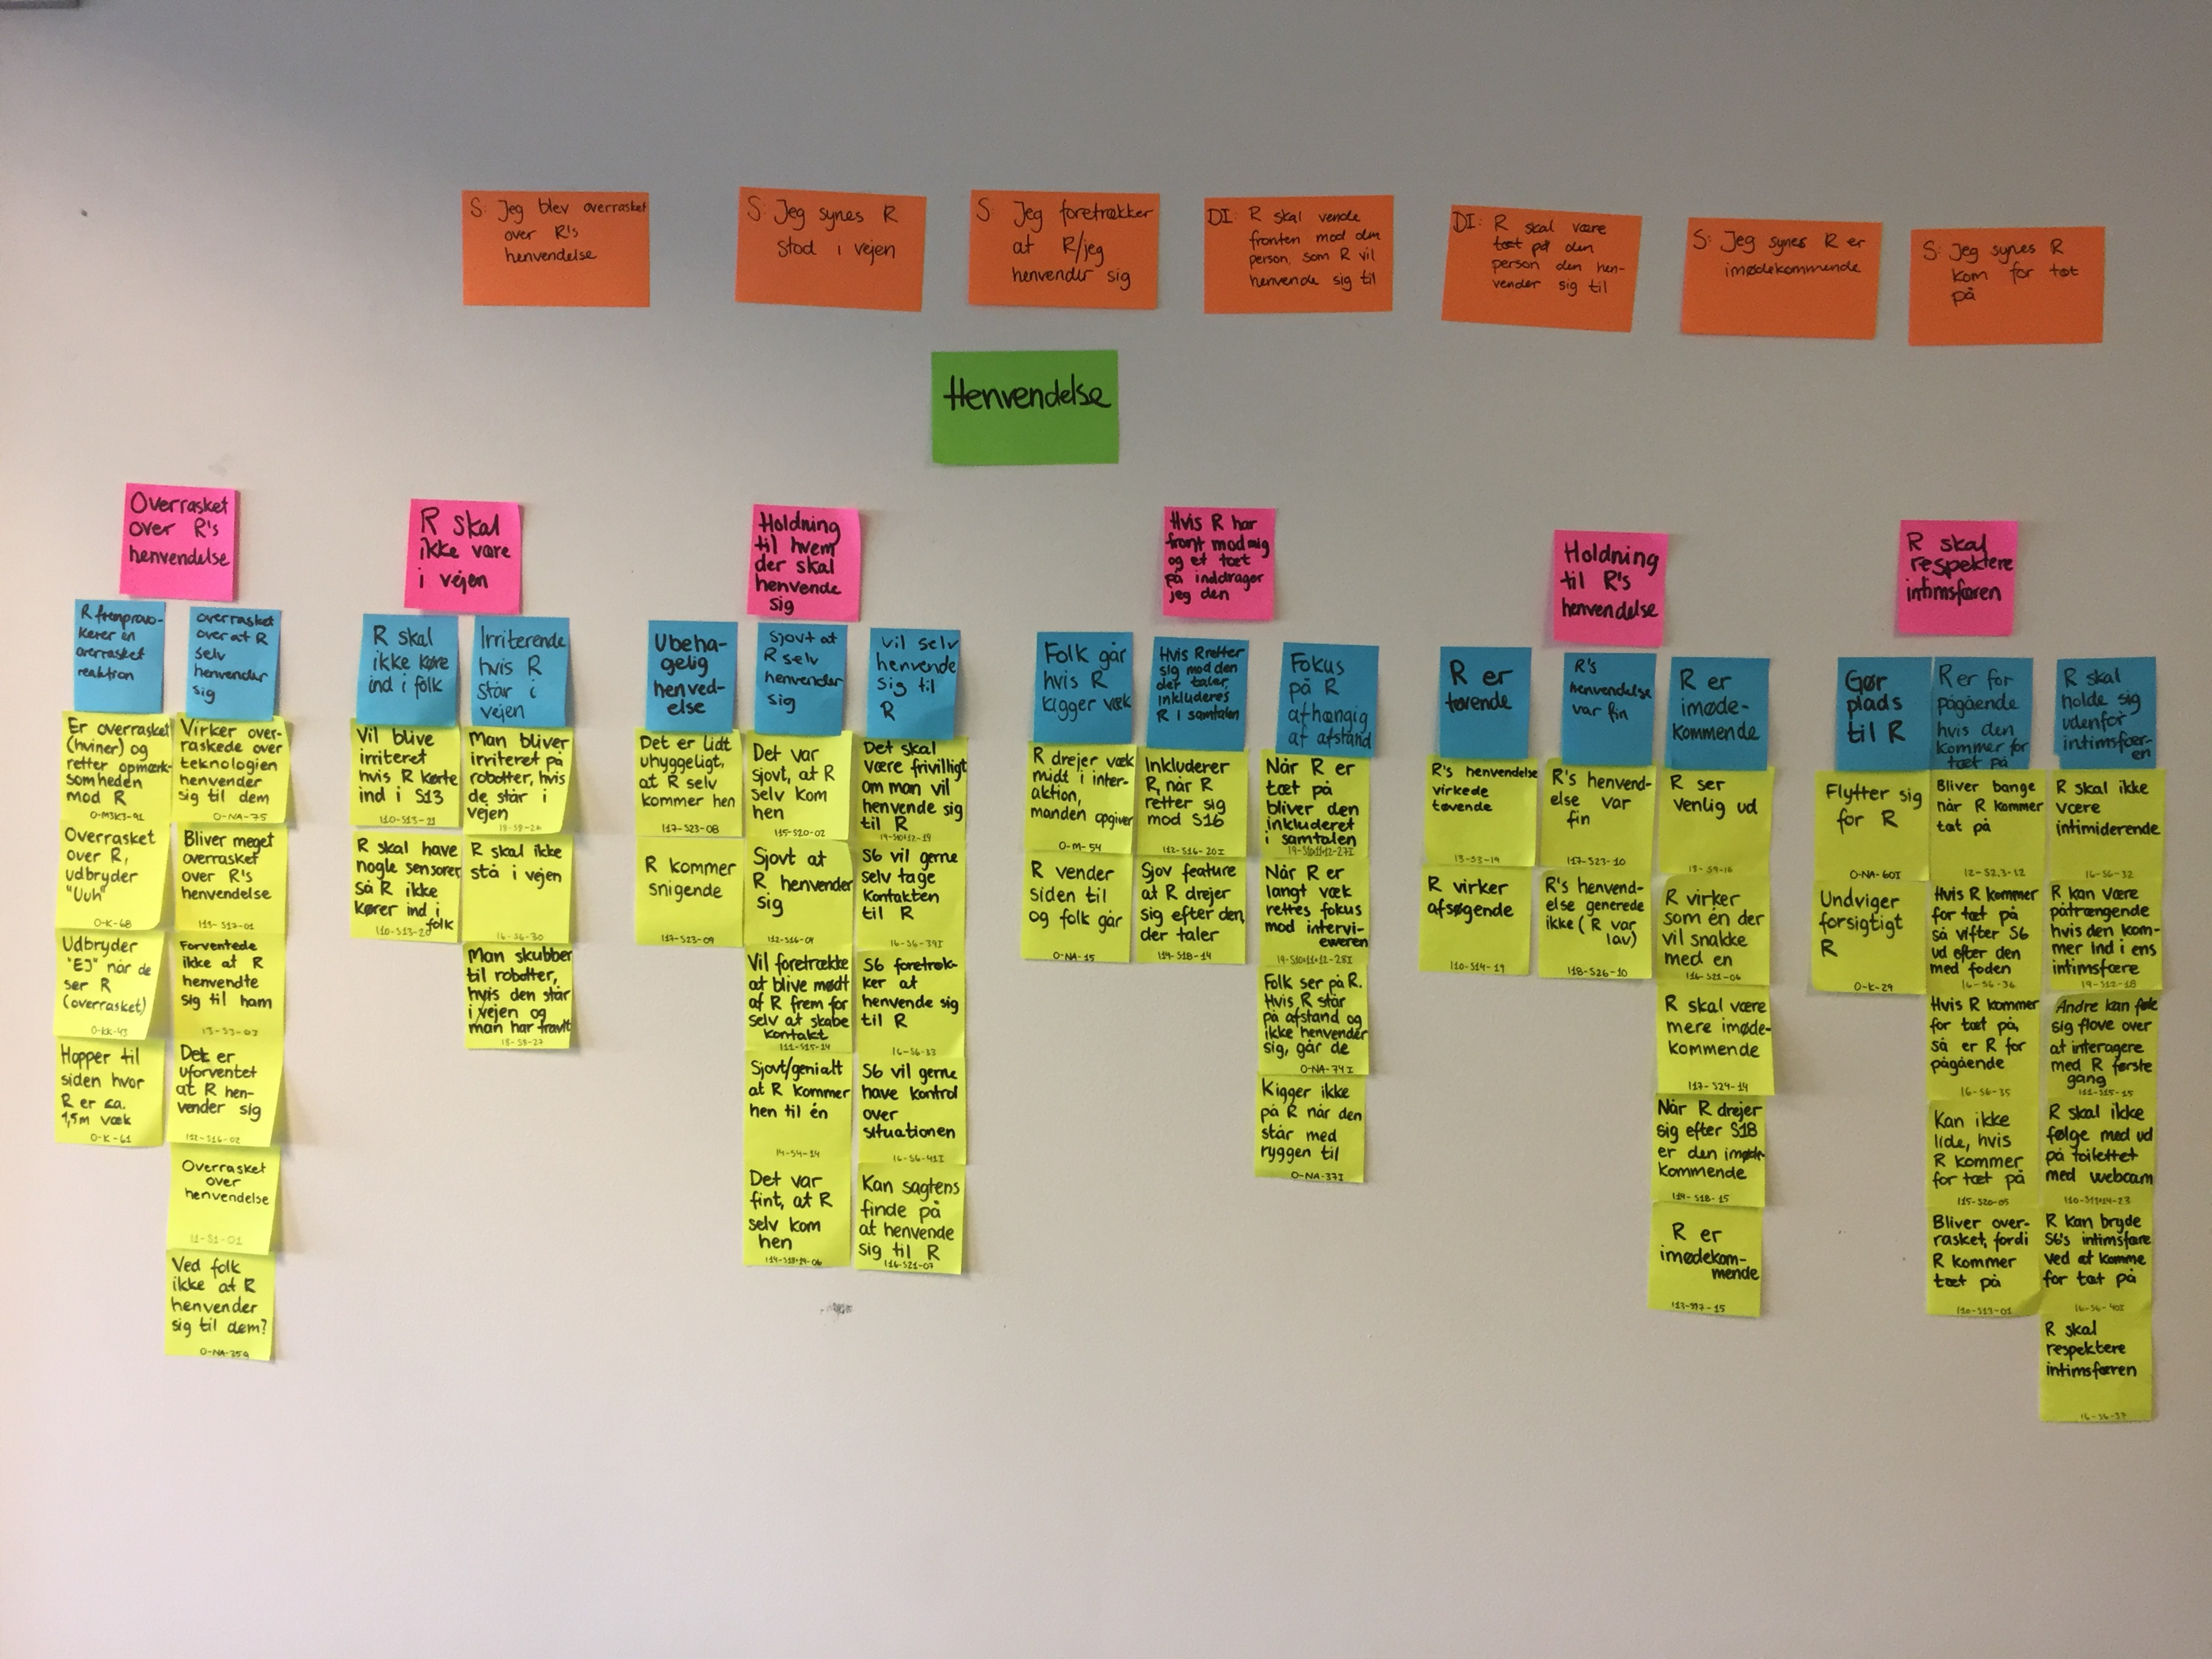
\includegraphics[width = 0.9\textwidth]{Figure/AffinityDiagram/Henvendelse} 
\caption{Oversigt over den grønne kategori: \textit{Henvendelse} med tilhørende \textit{affinity notes} placeret under henholdvist blå og pink labels, samt de udarbejde orange \textit{sticky notes}.}
\label{fig:AFHenvendelse}
\end{figure}
\noindent
\newpage
%
\subsection*{R's udseende}
%
\begin{figure}[H]
\centering
\includegraphics[width = 0.9\textwidth]{Figure/AffinityDiagram/RsUdseende} 
\caption{Oversigt over den grønne kategori: \textit{R's udseende}, hvor \textit{R} angiver robot, med tilhørende \textit{affinity notes} placeret under henholdvist blå og pink labels, samt de udarbejde orange \textit{sticky notes}.}
\label{fig:AFRsUdseende}
\end{figure}
\noindent
\newpage
%
\subsection*{Interesse for R}
%
\begin{figure}[H]
\centering
\includegraphics[width = 0.9\textwidth]{Figure/AffinityDiagram/InteresseForR} 
\caption{Oversigt over den grønne kategori: \textit{Interesse for R}, hvor \textit{R} angiver robot, med tilhørende \textit{affinity notes} placeret under henholdvist blå og pink labels, samt de udarbejde orange \textit{sticky notes}.}
\label{fig:AFInteresseForR}
\end{figure}
\noindent
\newpage
%
\subsection*{Positiv overfor R}
%
\begin{figure}[H]
\centering
\includegraphics[width = 0.9\textwidth]{Figure/AffinityDiagram/PositivOverforR} 
\caption{Oversigt over den grønne kategori: \textit{Positiv overfor R}, hvor \textit{R} angiver robot, med tilhørende \textit{affinity notes} placeret under henholdvist blå og pink labels, samt de udarbejde orange \textit{sticky notes}.}
\label{fig:AFPositivOverforR}
\end{figure}
\noindent
\newpage
%
\subsection{Kendskab til teknologi}
%
\begin{figure}[H]
\centering
\includegraphics[width = 0.9\textwidth]{Figure/AffinityDiagram/KendskabTilTeknologi} 
\caption{Oversigt over den grønne kategori: \textit{Kendskab til teknologi} med tilhørende \textit{affinity notes} placeret under henholdvist blå og pink labels, samt de udarbejde orange \textit{sticky notes}.}
\label{fig:AFKendskabTilTeknologi}
\end{figure}
\noindent
\newpage
%
\subsection*{Tillid til R}
%
\begin{figure}[H]
\centering
\includegraphics[width = 0.9\textwidth]{Figure/AffinityDiagram/TillidTilR} 
\caption{Oversigt over den grønne kategori: \textit{Tillid til R}, hvor \textit{R} angiver robot, med tilhørende \textit{affinity notes} placeret under henholdvist blå og pink labels, samt de udarbejde orange \textit{sticky notes}.}
\label{fig:AFTillidTilR}
\end{figure}
\noindent
\newpage
%